
\lhead[\chaptername~\thechapter]{\rightmark}

\rhead[\leftmark]{}

\lfoot[\thepage]{}

\cfoot{}

\rfoot[]{\thepage}

\chapter{Proposed Method}
\label{method}

% \begin{equation}
% \label{equa_model_potential}
% \small{
% \begin{aligned}
% \Psi(S^{(1)}, S^{(2)},J\mid G^{(1)}, G^{(2)}) &= \sum_{p\in\{1, 2\}} \Psi\sub{GO}(S^{(p)} \mid G^{(p)}) \\ &+\sum_{p\in\{1, 2\}} \Psi\sub{TS}(S^{(p)})\\
% &+\Psi\sub{JA}(J,S^{(1)},S^{(2)}\mid G^{(1)}, G^{(2)}) \\
% &+ \Psi\sub{TJ}(J),
% \end{aligned}
% }
% \end{equation}

\section{Hierarchical CNN}
\label{sec:HierCNN}

In the following subsections, we explain the process of building the hierarchy and CNN model. 
Then, we share the details of how we generate realistic training and test users.
Lastly, we define the baselines to compare with our method.

\subsection{Constructing the hierarchy}
\label{ssec:hierarchy}

According to our assumption, there is a high correlation between some pairs of classes in the sense that 
if users encounter a class, they are also likely to encounter another class if they are correlated. 
For example, in object recognition task, if users detect a computer, they are likely to detect a desk as well. 
By using this correlation, our objective is to place highly correlated classes closer in the hierarchy, 
so that users are most likely to find all the classes they need in nearby branches. 
As a result, users would use less branches and therefore less memory.

Given training user data that is described in subsection \ref{ssec:genusers}, we count the occurrences of class labels for each user. 
Secondly, we calculate the number of co-occurrences for every pair of class labels in the user data, obtaining a co-occurrence matrix.
Hierarchical distances between the class labels can be determined by inverting the ratios of the co-occurrence matrix, 
as the distance of two class labels is smaller when the number of co-occurences are larger. 
Applying hierarchical agglomerative clustering with the pre-calculated distances between each class label, we obtain a tree hierarchy as in the Figure \ref{fig:hierarchy}.

\begin{figure}
    \centering
    \begin{minipage}[b]{.4\textwidth}
        \centering
        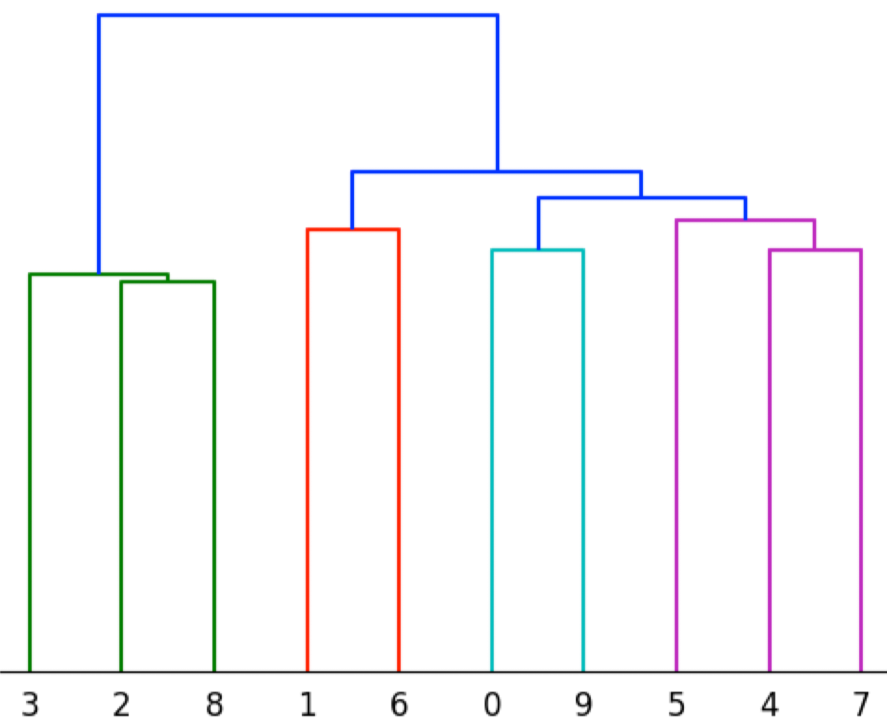
\includegraphics[width=.9\linewidth]{images/hierfig.png}
        %\caption{Hierarchical clustering of each class label in a 10-class example}
        \label{fig:sub1}
    \end{minipage}%
    \begin{minipage}[b]{.4\textwidth}
        \centering
        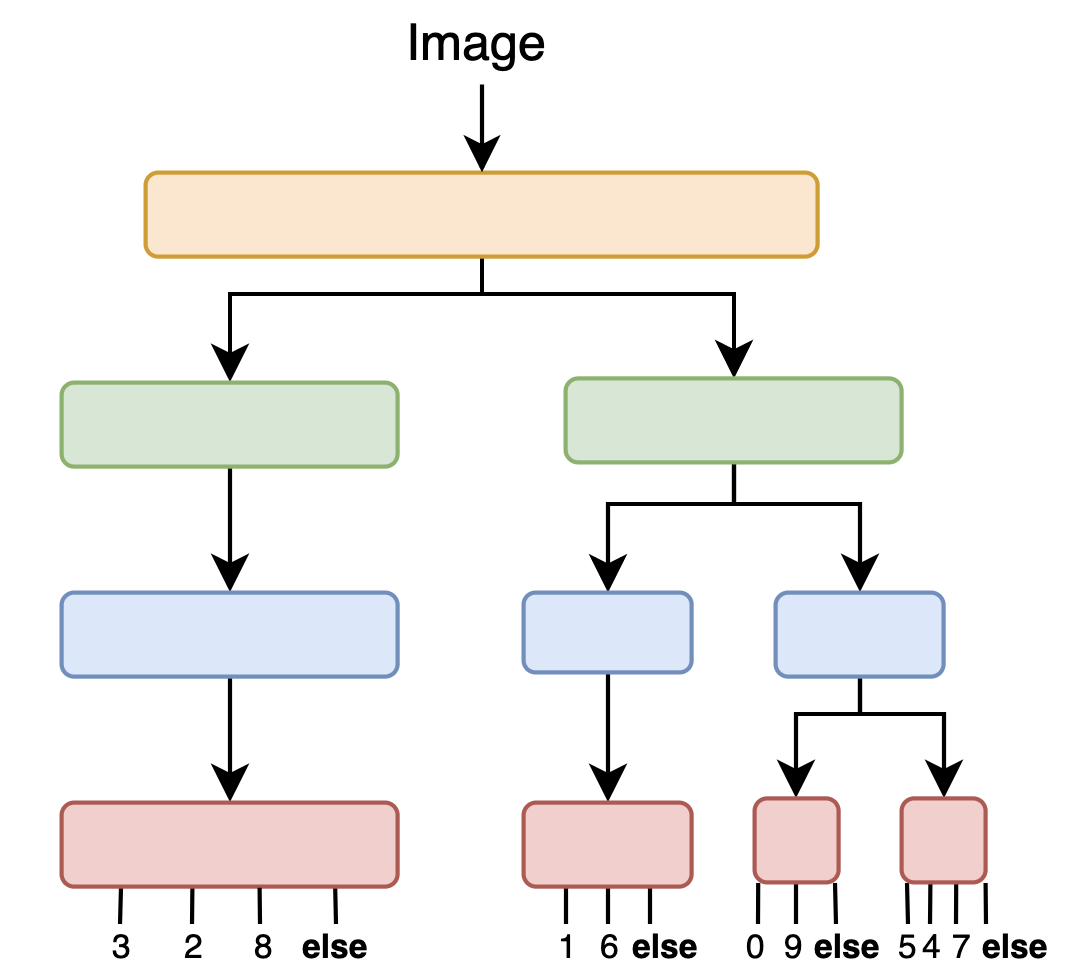
\includegraphics[width=.9\linewidth]{images/example_hier.png}
        %\caption{Hierarchical CNN obtained from the hierarchy on the left}
        \label{fig:sub2}
    \end{minipage}
    %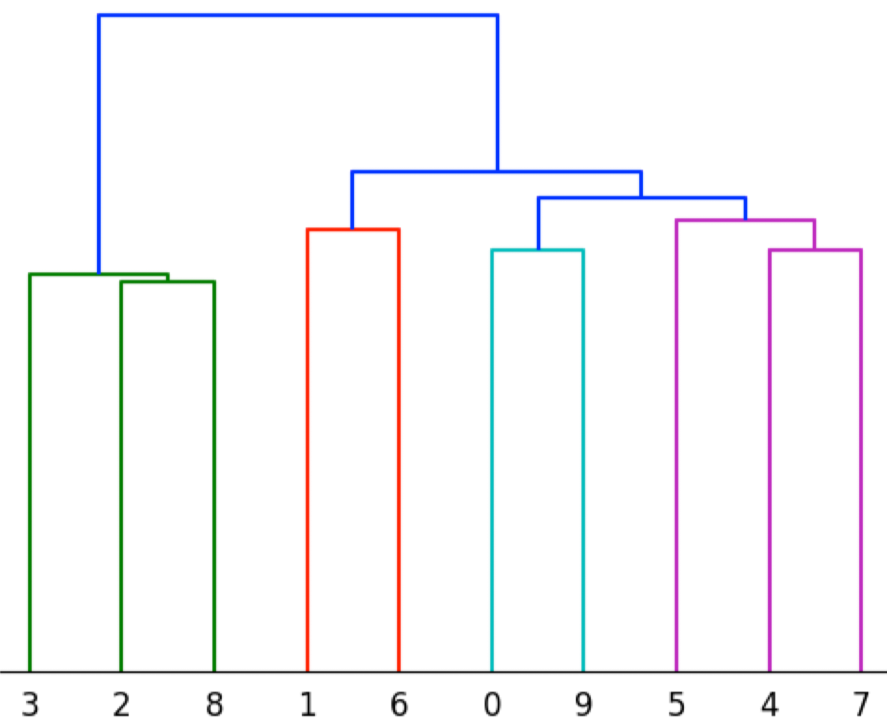
\includegraphics[width=0.40\textwidth]{images/hierfig.png}
    \caption{Hierarchical clustering of each class label in a 10-class example and the resulting network structure}
    \label{fig:hierarchy}
\end{figure}

\subsection{Hierarchy to CNN model}

Obtaining the hierarchy as described in \ref{ssec:hierarchy}, we construct our hierarchical CNN model. Depending on the hyper-parameters, such as depth of the tree, branching positions etc., there are many ways to construct the structure of hierarchical CNN with reference to the obtained hierarchy.

The structure is designed as a tree-shaped CNN, where the input image enters through the root layer.
Each layer takes the result of its parent layer as input and forwards its output to the next layer. 
Following the final output of the leaf layer is the classification layer for the subset of classes corresponding to that specific leaf, obtained from the hierarchy.
Note that, an extra classification label called 'else' is added to each leaves to detect classes that do not belong to a specific branch.
In real-life scenario, if a user's model gives the output 'else', it means the encountered image has the class label that the user's model does not include.  
Therefore, additional model parts are downloaded until the image is recognized.

When constructing the tree-structured CNN, we followed some constraints as follows. 
In general, tree-structured CNN is designed by following a backbone network, such as VGG16 or MobileNet, as the base network, and branching it recursively to obtain a tree version of the network.
The structure is designed to be a binary tree, meaning a layer can only branch into two layers. 
Moreover, every path from the root to each leaf follows the same order of layers, matching with the layer order of the backbone network.
Finally, the size of the resulting tree-structured CNN and the corresponding backbone network must be comparable. 
The reason is that if users end up using the entire tree-structured CNN, they would require only as much storage as the backbone network.
To achieve this, after each and every branching, the number of convolutional channels in the following layers are reduced.

There are also hyper-parameters that affects the structure of the tree-based CNN. 
'Depth' hyper-parameter controls the number of times that the network can branch into two following networks. 
On the other hand, 'branching positions' changes where the branching happens.
For example, if the first position is '3', the network branches just before the 4th convolutional layer in the backbone network.

In the light of all the above-mentioned constraints and hyper-parameters, the hierarchical CNN is constructed as in the figure \ref{fig:hierarchy}. 
In this simple example, the backbone network consists of four subsequent convolutional layer modules. 
'Depth' is set as 3 and 'branching positions are set as 1,2,3. 
Note that, reduced number of convolutional channels are represented as the size of the layers in the figure.
As an implementation rule, we do not split the branch if the remaining class labels in the branch is 3 or less. 
That is why the left branch in the figure is not divided into further sub-branches.

\subsection{Generating user types and case study users}

\label{ssec:genusers}

We require training and test users to create the hierarchy of our model and also test the final model in a scenario-based approach. 
Generated user data needs to be realistic as we chose to artificially generate the user data.

In our work, we assume that users interact with some classes significantly more than they interact with others due to their surroundings. 
Therefore, we defined a number of user types, each following a Dirichlet distribution, 
which the parameters of the distributions are selected to prioritize a subset of the classes. 
All users are generated according to one of the user type distribution. 
The user types can be interpreted as people with different surroundings, 
for example a chef is surrounded by kitchen tools whereas a pilot encounters airplanes on a daily basis.

When defining user types as Dirichlet distributions, we randomly put high values(200s) for high likely to encounter classes and low values(1s) for less likely to encounter classes. For example, a user type in 5-class classification would be $Dir(1,1,200,1,200)$. 
A test user generated from this specific distribution will encounter images in 3rd and 5th class much more than the rest of them. 
We chose the number of high values(200s) in a user type as 2 or 3 for testing CIFAR-10, which means each user is likely to encounter 2 or 3 classes out of 10 classes. 

To generate a user, a user type is chosen uniformly randomly between $m$ user types. 
Then, list of encountered class labels for the user are generated according to the chosen user type. 
An example of list of encountered class labels would be, $(3,3,5,3,5,5,...,2,...,3,5,3)$ if generated from the distribution $Dir(1,1,200,1,200)$. 
It can be interpreted as the user usually encounters 3rd and 5th classes and sometimes encounters other classes as well.
Finally, random images from the dataset are collected corresponding to the class categories in the list to make a scenario-based test set for the user.

On a final note, training users are generated to construct the hierarchy of the system, whereas test users are generated to test our model as a scenario-based approach. 
Both training and testing users are from the same user types as we assume correlation between the requirements of all users. 

\begin{figure}
    \centering
    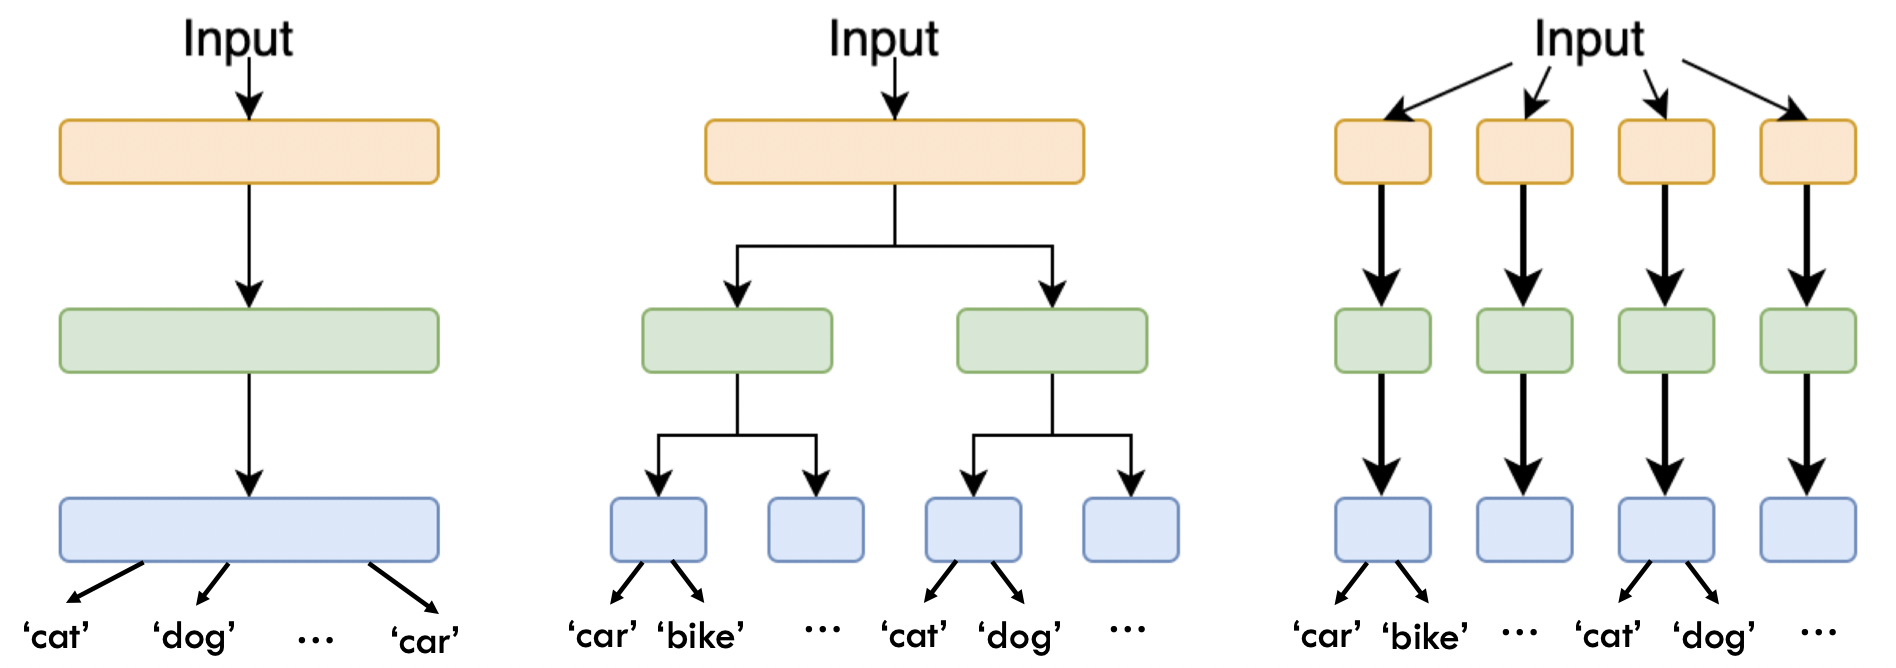
\includegraphics[width=0.9\textwidth]{thesis/images/classification_baselines-fig.png}
    \caption{Left is the regular CNN model. Middle one is the proposed hierarchical CNN. Right is the multiple smaller regular CNNs. Note that, all models are comparable in size.}
    \label{fig:baselines}
\end{figure}

\subsection{Baselines}
\label{ssec:baselines}
The whole network size of the hierarchical CNN and the baseline networks are approximately equal, because it would be fair to compare the networks with similar number of parameters. 
We constructed the hierarchical CNN simply by following a backbone network's layer order and splitting into sub-branches according to the obtained hierarchy. 

Another straightforward approach to our problem is using multiple backbone networks each reduced in size with the task of classifying a subset of classes. 
These subsets of classes corresponds to the same subsets of classes recognized in the leaf nodes of hierarchical CNN.
Same as the hierarchical CNN, we reduce the size of the each network to make the total sum of the number of parameters of all networks equal to the backbone network. 
We will refer to this method as multiple CNNs. 

In this method, none of the networks share parameters, thus decreasing the size of each network more than that of hierarchical CNNs by also reducing the number of parameters in the earlier layer. 
However, reducing the number of extracted low-level features from the input image in the early layers would result in a decrease of accuracy. 
The decrease in the accuracy is dire especially when the number of sub-networks is higher because we reduce the size of the each network more to balance with the backbone network size. 
We compare both the methods and the backbone network in terms of their accuracy and average memory consumption per user. 
All three architecture can be seen in the figure \ref{fig:baselines}.


\section{Faster ANN}
\label{sec:FasterANN}

\begin{figure}
    \centering
    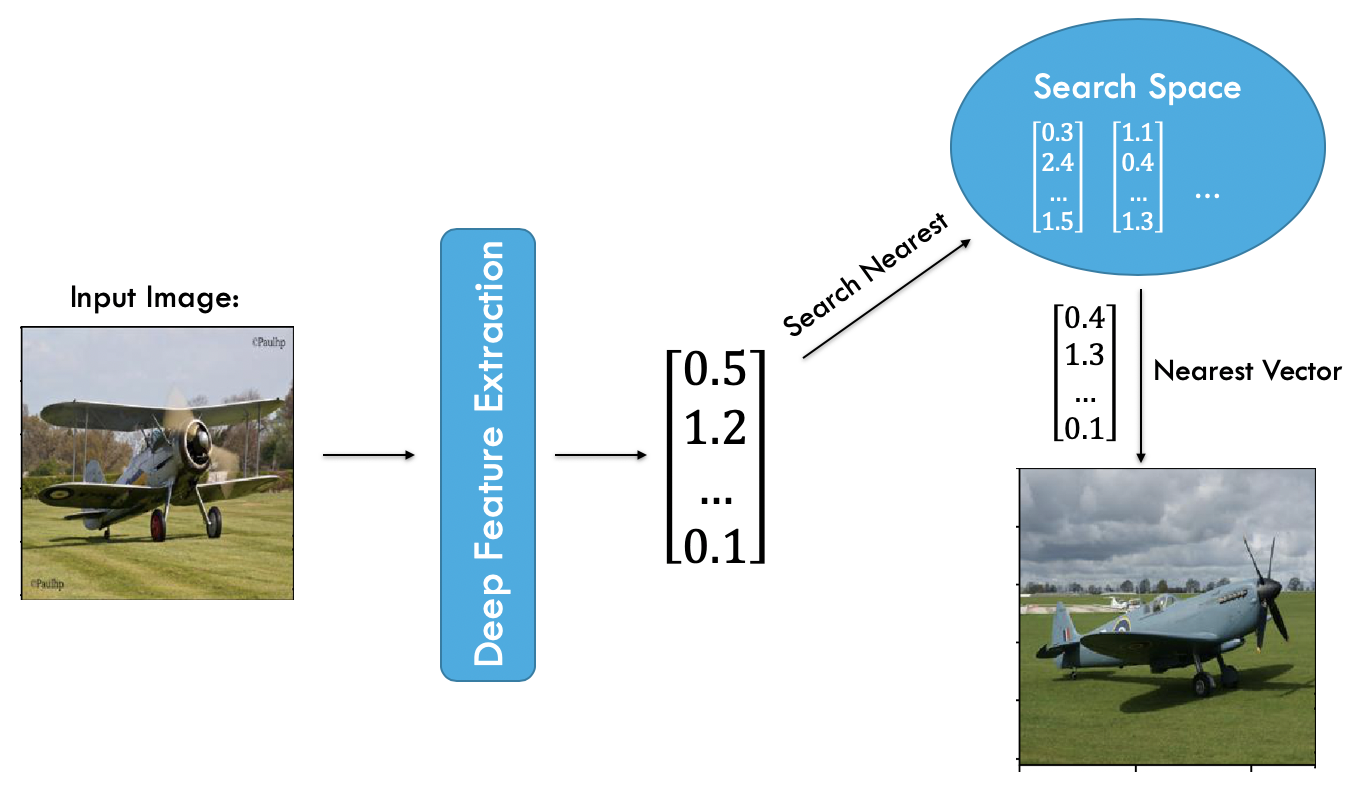
\includegraphics[width=0.9\textwidth]{thesis/images/image_ret_exp-fig.png}
    \caption{Overview of Image Retrieval}
    \label{fig:ret-exp}
\end{figure}

Image retrieval task consists of two tasks, representing images with vectors and searching a database of vectors for the nearest vector to the input image, as in figure \ref{fig:ret-exp}. 
Naive approach would be brute-force searching the entire database.
However, exhaustive searching of the database is slow and complex, especially with vectors with large dimensions. 
Thus, Approximate Nearest Neighbor (ANN) search algorithms are proposed with significantly faster search speed and a small probability of error. 
We built our work on the FAISS implementation\cite{faiss} of Product Quantization\cite{jegou2010product} with inverted multi-index as well as using it as our baseline.

As explained previously in \ref{subsec:related-quantization}, product quantization method clusters the database space into $k$ clusters using k-means clustering algorithm. 
Following the convention, we chose $k=\sqrt{N}$ where $N$ is the number of database vectors. 
In this way, number of vectors corresponding to a centroid of a cluster will be $\sqrt{N}$ in average. 
Once a query vector comes, the algorithm searches the closest centroid among $\sqrt{N}$ centroids. 
Then, the query vector is compared with the database vectors that belong to the chosen centroid and a few neighboring ones. 
In both steps, there are $O(\sqrt{N})$ comparisons to be done. 

Our work aims to reduce the number of comparisons in the first step by limiting the area of the search space for each user according to their requirements. 
The motivation is that most users have a certain query distribution, different than that of the database, 
so they query some parts of the search space more and the other parts less likely. More will be explained in \ref{motivation}.

In the following subsections, methods of our work will be explained in detail. 
Firstly, the motivation of our idea will be discussed.
Then, method of representing the images with vectors will be described. 
Next, the details of the dataset we used and the importance of using classification label information for our work will be explained. 
After specifying the implementation details, baselines of our work will be defined.

\subsection{Motivation}
\label{motivation}

\begin{figure}
    \centering
    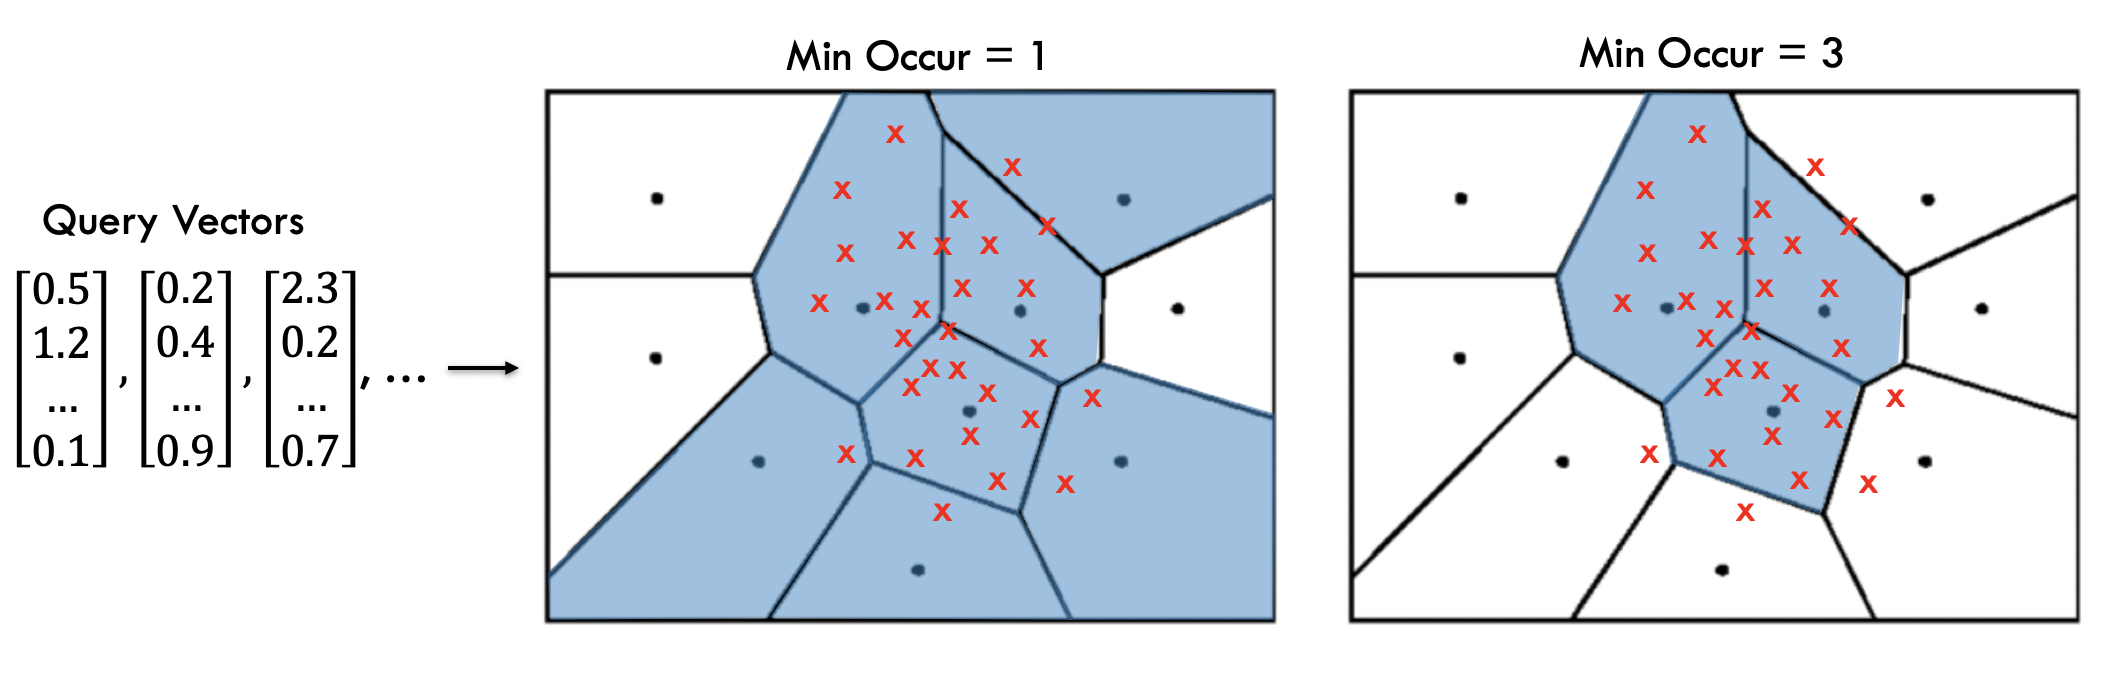
\includegraphics[width=\textwidth]{thesis/images/improvement-fig.png}
    \caption{Query vectors and clustering of the search space is shown. Red crosses represent the position the query vectors fall in the space. We can choose to include every subspace with red crosses in our search as in the left figure. A hyper-parameter can control to include a subspace according to minimum occurrence of red crosses.}
    \label{fig:motivation}
\end{figure}

ANN search algorithms commonly assume that the distribution of the query vectors is the same with the distribution of the database. 
However, real users query the system with different distributions.
This difference is sourcing from their limited surroundings in daily life or their different hobbies and interests. 
By utilizing this idea, we can reduce the search space for each user according to their requirements.

In figure \ref{fig:motivation}, an example of query images are coming from a user is shown with red crosses on the search space. 
For this user, a new query vector just needs to be compared with centroids in blue areas. 
We can reduce the amount of centroids to compare with a simple hyper-parameter, controlling whether to include a subspace according to minimum occurrence of the past query vectors. 
In this way, we can adjust the trade-off between accuracy and the speed of the system.


\subsection{Extracting Deep Features of Images}

\begin{figure}
    \centering
    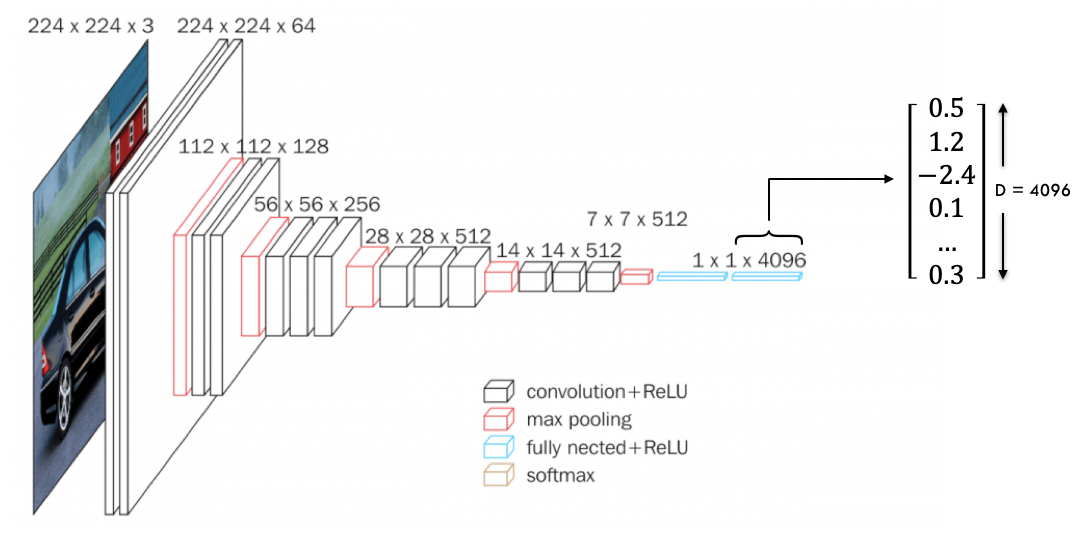
\includegraphics[width=0.9\textwidth]{thesis/images/deep_features-fig.png}
    \caption{Last fully connected layer of VGG16\cite{simonyan2014very} is discarded to obtain a descriptor vector with dimension 4096.}
    \label{fig:vec-repr}
\end{figure}

In the work of Babenko \emph{et al.}\cite{babenko2014neural}, using a pre-trained convolutional neural network in ImageNet for image retrieval task is shown to have decent results. 
Note that, it is also shown that if the network is trained on the same data with the retrieval dataset, the results are better.
However, instead of getting the best performance, we simply investigate the comparison of our idea with the current best methods.
Therefore, we used VGG16\cite{simonyan2014very} network that is pre-trained on ImageNet\cite{deng2009imagenet}. 
The last fully connected layer is discarded to get a vector representation with 4096 dimensions, as in figure \ref{fig:vec-repr}.
Then, all database images are passed through the model once to get their descriptor vectors.

However, dimensions of the vectors were quite big for both storage and calculation. 
As stated in \cite{jegou2012negative}, applying whitening on the descriptor vectors not only helps with the computational and storage costs, but also improves the accuracy of retrieval tasks.
We applied Principal Component Analysis (PCA) to obtain the final descriptor vectors with 64 dimensions.


\subsection{Dataset and Using classification label information}

In our experiments, we used the scene recognition dataset called Places365\cite{zhou2017places}. 
Only the training images of Places365 is used to construct our retrieval database. 
There are 1.8 million training images with 365 class categories. 
The class categories include various scenes such as airport terminal, library, train station, waterfall, etc. 
With such diverse scenes, users would interact with only a subset of the class categories and our idea can be easily applied to speed up the search according to each user's requirements.

\begin{figure}
    \centering
    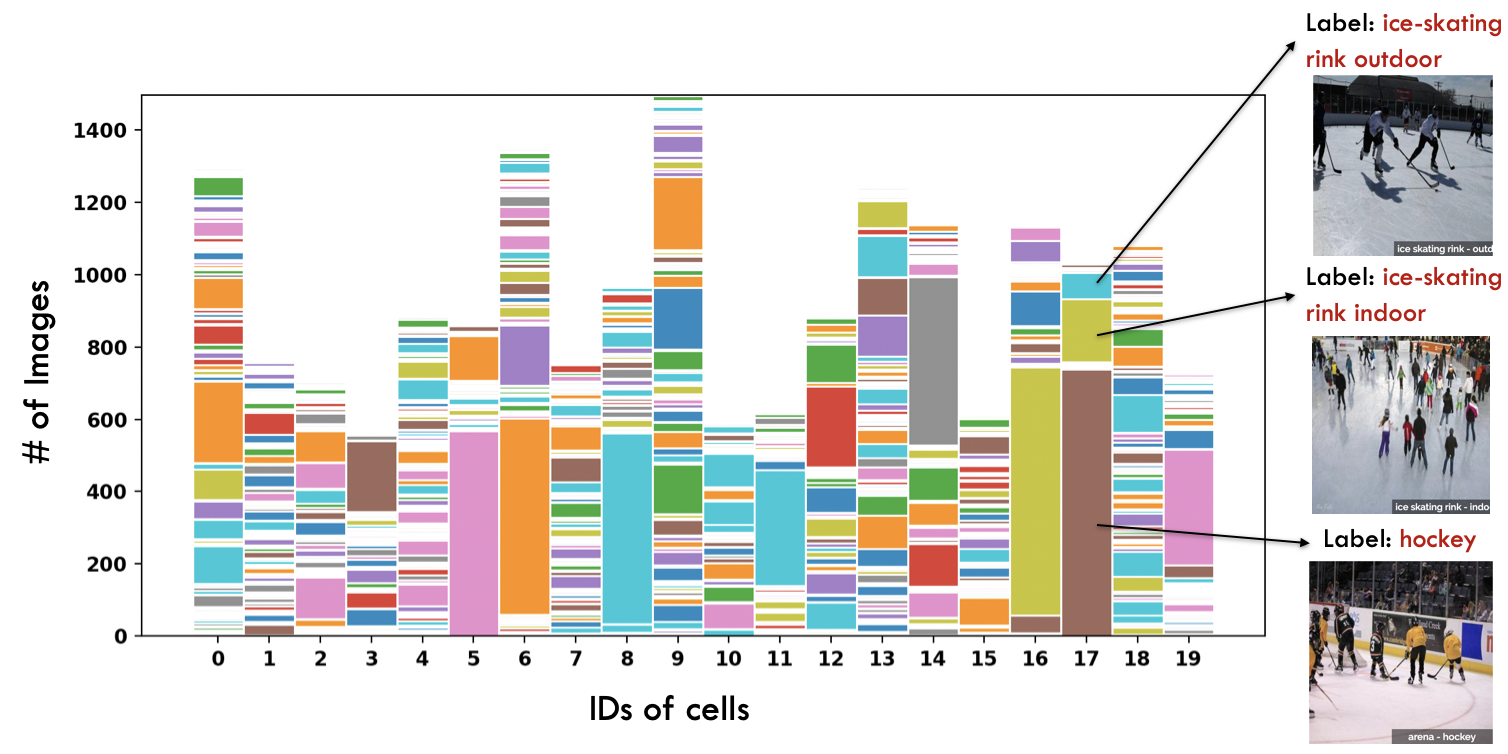
\includegraphics[width=\textwidth]{thesis/images/label_dist-fig.png}
    \caption{Distribution of the images according to their class labels in the first 20 subspaces}
    \label{fig:label-dist}
\end{figure}

The search space is divided into 1350 subspaces which is roughly the square root of the number of all images. 
Distribution of the images according to their classification labels can be seen in the figure \ref{fig:label-dist}.
As can be seen in the figure, some subspaces have extreme bias towards a few class, while others do not have much. 
There are many class categories in Places dataset that have similar images, such as "elevator-door", "elevator-interior", "elevator lobby", "elevator shaft", etc.
For example, the subspace with id:17 in the figure has labels with very similar images.

According to our scenario, users have wearable devices with a camera, such as wearable glasses or a smart phone. 
When they first start using the image search system, the class recognition system will store the classification labels of the users. 
After storing labels for enough time, we will consider those labels as the user's required class labels.
Then, we select the subspaces, out of all 1350 subspaces, that contain any of those class labels at least $m$ times. 
$m$ is the hyper-parameter to adjust the trade-off between accuracy and speed.
Whenever a new query image comes from the user, we compare the query vector only with the centroids of the selected subspaces to reduce time.
Note that, classification labels are merely a tool for us to categorize the requirements of the users.
Most similar images do not necessarily have the same labels.


\subsection{Implementation details}

As mentioned before, we built our work on FAISS implementation\cite{faiss} of product quantization with inverted index, namely IndexIVFPQ. 
The code is shared publicly and we modified the code to tailor to our needs.
Extra function is added to adjust the search space according to a given list. 
This function is called during the indexing phase of the database before the search.

The training phase is required for IndexIVFPQ and it needs different vectors than the database vectors with similar distribution.
Training dataset of Places365 contains 1.8 million images. 
After obtaining the descriptor vectors of the images, we split the vectors into three parts.
Base vectors containing roughly 1.3 million vectors to form the search space, about a half million training vectors to train IndexIVFPQ and remaining approximately 3000 for query vectors.
The vectors are split into 3 parts in a way that the number of images for each label in all parts are almost equal.
When querying for a user, only the images with the required labels out of 3000 are used for the query images when mimicking scenario users.

\subsection{Baselines}

Our main baseline is the FAISS implementation\cite{faiss} of product quantization with inverted index, namely IndexIVFPQ.
We compared our method with IndexIVFPQ by evaluating for search time per query and recall at 1 where recall at $k$ checks if the true result is one of the $k$ predicted results.

